\documentclass{article}
\usepackage{nips07submit_e,times}
\usepackage{graphics}
\usepackage{graphicx}
\usepackage[small,hang]{caption}
\usepackage{amsmath,amsfonts,amsthm,amssymb}
\usepackage{Tabbing}
\usepackage{fancyhdr}
\usepackage{chngpage}
\usepackage{soul,color}
\usepackage{float,wrapfig}
\usepackage{multirow}
\usepackage{enumerate}
\usepackage{alltt,comment}
\usepackage{fixltx2e}
%\documentstyle[nips07submit_09,times]{article}

\title{Technical Report:\\ME Algorithm for Hierachical Dirichilet Process}
\author{}
\newcommand{\fix}{\marginpar{FIX}}
\newcommand{\new}{\marginpar{NEW}}

\begin{document}
\makeanontitle

\begin{abstract}We here develop a Maximize-Expectation(ME) learning algorithm for Hierarchical Dirichilet Process(HDP).
We first show the advantage of ME algorithm over other varitional methods to learn Dirichlet Process Mixture model(DPM) as a baseline. 
Then we use Chinese Restaurant Franchise(CRF) representation to construct ME algorithm for HDP, which 
gives reasonable results on synthetic data. 

\end{abstract}

\section{Introduction}
\subsection{Dirichilet Process Models}
\subsubsection{Dirichilet Process Mixture}
In probability theory, the Dirichlet process DP($\alpha_{0},G_{0}$) is a measure on measures, where $\alpha_{0}$ is a scaling
parameter and $G_{0}$ is a base probability measure. 
If $G_{0}$ is a finite measure and X is a random distribution drawn from a Dirichlet process, written as $X \sim \mathrm{DP}\left(\alpha,G_{0}\right)$
then for any partition of the probability space $\left\{B_i\right\}_{i=1}^{n}$, we have that
$\left(X\left(B_1\right),\dots,X\left(B_n\right)\right) \sim \mathrm{Dirichlet}\left(\alpha_{0}G_{0}\left(B_1\right),\dots,\alpha_{0}G_{0}\left(B_n\right)\right)$.
Also, we have the following stick-breaking representation:
\begin{eqnarray*}
 G=\sum_{k=1}^{\infty} \beta_{k}\delta_{\phi_{k}}
\end{eqnarray*}
where the $\phi_{k}$ are the independent random variables distributed accoring to $G_{0}$,
$\delta_{\phi_{k}}$ is an atom at $\phi_{k}$
and $\beta_{k}$ are the stick-breaking weight depending on the parameter $\alpha$.\\
\begin{eqnarray*}
\phi_{k}|G_{0}\sim G_{0}\\
v_{k}|\alpha \sim Beta(1,\alpha)  & for & k = 1,...,\infty\\
\beta_{k}=v_{k}\Pi_{l=1}^{k-1}(1-v_{l})
\end{eqnarray*}
In recent years, Drichilet process mixture model has become popular for clustering problems in Nonparametric Bayesian literature. 
It gracefully avoids to determine the number of clusters beforehand, which has haunted previous methods like K-means to Latent Dirichlet Allocation(LDA).
\subsubsection{Hierarchical Dirichilet Process}
The hierarchical Dirichlet process (HDP) is useful in problems in which there are multiple groups of data, where the model for each group of data incorporates a discrete variable of unknown cardinality, 
and where we wish to tie these variables across groups (Teh et al., 2006).
For example, in document modeling, the aim is to cluster words within the documents into different topics. 
When clustering documents from NIPS in machine learning and  computer vision, 
we may wish to allow topics like \textquotedblleft graphical model \textquotedblright and \textquotedblleft optimization\textquotedblright to be shared among them.\\ 

The basic building block of a hierarchical Dirichlet process is a recursion in
which the base measure $G_{0}$ for a Dirichlet process G $\sim$ DP($\alpha$, $G_{0}$) is itself a draw
from a Dirichlet process: $G_{0}\sim$ DP($\gamma$,H). This recursive construction has the
effect of constraining the random measure G to place its atoms at the discrete
locations determined by $G_{0}$ . The major application of such a construction is to
the setting of conditionally independent hierarchical models of grouped data.
More formally, consider an indexed collection of DPs, $\{G_{j}\}$, one for each of a
countable set of groups and defined on a common probability space ($\Theta$, $\Omega$). The
hierarchical Dirichlet process ties these random measures probabilistically by
letting them share their base measure and letting this base measure be random:
\begin{eqnarray*}
 & &G_{0}|\gamma,H \sim DP(\gamma,H)\\
\forall j & &G_{j}|\alpha_{0},G_{0} \sim DP(\alpha_{0},G_{0}) 
\end{eqnarray*}
\subsubsection{Pitman-Yor Process and Hierarchical Pitman-Yor Process}
The Pitman-Yor process is a two-parameter generalization of the DP, with a discount parameter 0 $\leq$ d $<$ 1 and a concentration parameter $\alpha>$ −d. 
When d = 0, the Pitman-Yor process reduces to a DP with concentration parameter $\alpha$. 
We write G $\sim$ PY(d, $\alpha$, H) if G is a Pitman-Yor process with the given parameters and base measure H.
The stick-breaking construction and the Chinese restaurant process have natural generalizations in the Pitman-Yor process. 
A draw G from the Pitman-Yor process has the following stick-breaking construction:
\begin{eqnarray*}
 G=\sum_{k=1}^{\infty} \beta_{k}\delta_{\theta_{k}}
\end{eqnarray*}
Where:
\begin{eqnarray*}
\theta_{k}|G_{0}\sim G_{0}\\
v_{k}|d,\alpha \sim Beta(1-d,\alpha+kd)  & for & k = 1,...,\infty\\
\beta_{k}=v_{k}\Pi_{l=1}^{k-1}(1-v_{l})
\end{eqnarray*}
The hierarchical Pitman-Yor (HPY) process is defined in the obvious manner:
\begin{eqnarray*}
 & &G_{0}|\gamma,H \sim PY(\gamma,H)\\
\forall j & &G_{j}|\alpha_{0},G_{0} \sim PY(\alpha_{0},G_{0}) 
\end{eqnarray*}

\subsection{ME Algorithm}
Consider a probabilistic model P(x,w,$\alpha$),where x is observed random variable, w hidden variable and $\alpha$ hyperparameter.   
For the generative approach to clustering problem, hidden variables are divided into two classes: cluster assignment z and generative model parameters $\theta$.  
The typical task in machine learning is to estimate the distribution of hidden variable w: p(w$|\alpha$)=p(z,$\theta|\alpha$).
For variational methods, the goal is to find the estimation q(z,$\theta$) that minimizes the KL divergence from posterior distribution $p(z,\theta |\vec x,\alpha)$, which 
is equivalent to maximizing the lower bound $\mathcal{L}(q(z,\theta))$ for the likelihood:
\begin{eqnarray*}
log p(\vec x |\alpha)
&\geq&\mathcal{L}(q(z,\theta)) \\
&=&log p(\vec x | \alpha)-KL[q(\theta,\vec z) || p(\theta,\vec z | \vec x,\alpha)] \\
&=&-\boldmath{E}[log p(\vec x,\vec z, \theta | \alpha)]_{q(\theta,\vec z)}-H[q(\theta,\vec z)] 
\end{eqnarray*}
where $H(q(w))=-\int_w \ q(w)log [q(w)] dw$ is the entrophy.
Instead of estimating the joint distribution q(z,$\theta$), the normal approach is to factorize it into q(z)q($\theta$) which can be updated iteratively as coordinate ascent. 
In general, we can either maintains distribution estimation(known as E-step) or point estimation(known as M-step) for the hidden variable.
The popular Meanfield method iteratively estimates the disribution for z and $\theta$ with the following formula.
\begin{center}
$q (\theta ) \propto exp(E[log P(\theta, z, D)]_{q(z)} ) \longleftrightarrow q (z) \propto  exp(E[log P(\theta, z, D)]_{q (\theta )})$.
\end{center}
In contrast, K-means algorithm keeps a point estimation for both $\theta$ and z. 
Discussed in [4], we can have four different combinations of E-step and M-step for z and $\theta$. 
For our interest, we find ME algorithm(M-step for z, E-step for $\theta$) suitable for the clustering problem for the following reasons:
\begin{enumerate}
 \item In pratice, people may just want the optimal solution for the cluster assignment z instead of the real distribution of q(z).
Thus point estimation for z is enough
 \item For most of the time, the cluster assignment z is discrete and high dimensional, which makes the update formula non-analytic and hard to approximate.
\end{enumerate}
Thus the learning problem is transformed into a combinatorial optimizaiton problems, which we plan to solve with heuristic searching algorithms.

\section{Motivation: A quick comparison of algorithms on DP Mixture Model}
Before diving into the details of complicated hierarchical models, we first test variants of ME algorithm for the simpler DP-Mixture model with Gaussian conjugated with Normal-Inverse-Wishart(NIW) distribution.
\subsection{Formula}
Let $x_{n}$ , $\left[n=1,...,N\right]$, be a vector of independent and identically distributed continuous-valued observations in D dimensions. 
For each data case, we define a cluster assignment variable, $z_{n}\in \left[1, . . . , K \right]$.
Assuming that the data have been generated following a mixture of gaussians, we place the standard conjugate priors on the parameters:
\begin{eqnarray*}
p(x_{n},z_{n},\theta)=\{\mathcal{N}(x_{n}|z_{n},\mu,\Omega)\mathcal{N}(\mu|m_{0},\xi_{0}\Omega)\mathcal{W}(\Omega|\eta_{0},B_{0})\}\{\mathcal{M}(z_n|\phi_{0}\mathcal{D}(\phi_{0}|\lambda)\}
\end{eqnarray*}
Thus the log-likelihood: 
\begin{eqnarray*}
log(p(x,z|\lambda))
&=&-\frac{D N}{2}log\pi-\sum_{k=1}^{K} [\frac{D}{2}log\frac{\xi_{k}}{\xi_{0}}+\frac{\eta_{k}}{2}log det(B_{k})-\frac{\eta_{0}}{2}log det(B_{0})
-log \frac{\Gamma_{D}(\frac{\eta_{k}}{2})}{\Gamma_{D}(\frac{\eta_{0}}{2})}]\\
&+&log(\frac{\Gamma(\phi_{0})}{\Gamma(N+\phi_{0})})+\sum_{k=1}^{K}[log \Gamma(N_{k})+log\phi_{0}]\\ 
\end{eqnarray*}
where 
\begin{eqnarray*}
&&\phi_{k}=\phi_{0}+N_{k}\ \ \ m_{k}=\frac{N_{k}\bar x_{k}+\xi_{0}m_{0}}{\xi_{k}}\ \ \ B_{k}=B_{0}+N_{k}S_{k}+\frac{N_{k}\xi_{0}}{\xi_{k}}(\bar x_{k}-m_{0})(\bar x_{k}-m_{0})^{T} \\
&&\eta_{k}=\eta_{0}+N_{k} \ \ \ \xi_{k}=\xi_{0}+N_{k}\ \ \ \Gamma_{D}(x)=\pi^{\frac{D(D-1)}{4}}\Pi_{i=1}^{D}\Gamma(x+\frac{1-i}{2})
\end{eqnarray*}
$N_{k}$ number of datas in cluster k,$S_{k}$ the sample covariance in cluster k and $m_{k}$is the sample mean of cluster k



\subsection{Simple search algorithm}
The goal is to optimize the log-likelihood by searching over cluster assignment z in the discrete high dimensional space.
For ME learning algorithm, we here propose three basic search moves:
\begin{enumerate}[(a)]
\item Local Move: find the best cluster assignment for one data point at a time
\item Merge Move: find the best cluster for a certain cluster to merge
\item Split Move: use heuristic methods described in [4]to split one cluster into 2
\end{enumerate}
Here, we try four simple versions of ME algorithms:
\begin{enumerate}[(a)]
\item randomized local move until convergence
\item randomized local move until convergence+merge move once
\item Bayesian K-means(Hierarchical clustering)[4]
\begin{enumerate}[(i)]
 \item Bottom-Up: merge move
 \item Top-Down: split+ merge move
\end{enumerate}
\end{enumerate}
\subsection{Results on Synthetic Data}
We test Meanfield algorithm (EE) [1], Collapsed Meanfield algorithm(Collapsed-EE)[5] and ME algorithm [3] implemented by Kurihara on the synthetic data, 200 random samples drawn from Gaussian of four mixtures.
We set the same hyperparameters for these three algorithms and test with different initial cluster numbers.
Results are summarized in table 1. 
From figure 2 c),d), we can see that to some degree both EE and Collapsed EE suffer from local minimas.
For ME algorithms, even the naive local search+ merge works reasonably well.
Though Kurihara's Hierachical Clustering version of ME works perfect here, it's impractical in two folds:
\begin{enumerate}[(a)]
\item formula for HDP model is more complicated and conjugated distributions like Dirichlet-Multinomial may not have the strong spatial cue for the Gaussian case.
Thus, heuristic split-merge strategy will get stuck easily for advanced models.
\item For larger data set, split-merge here are global greedy methods which will lead to high complexity.
\end{enumerate}
\begin{figure}[h] 
    \centering 
    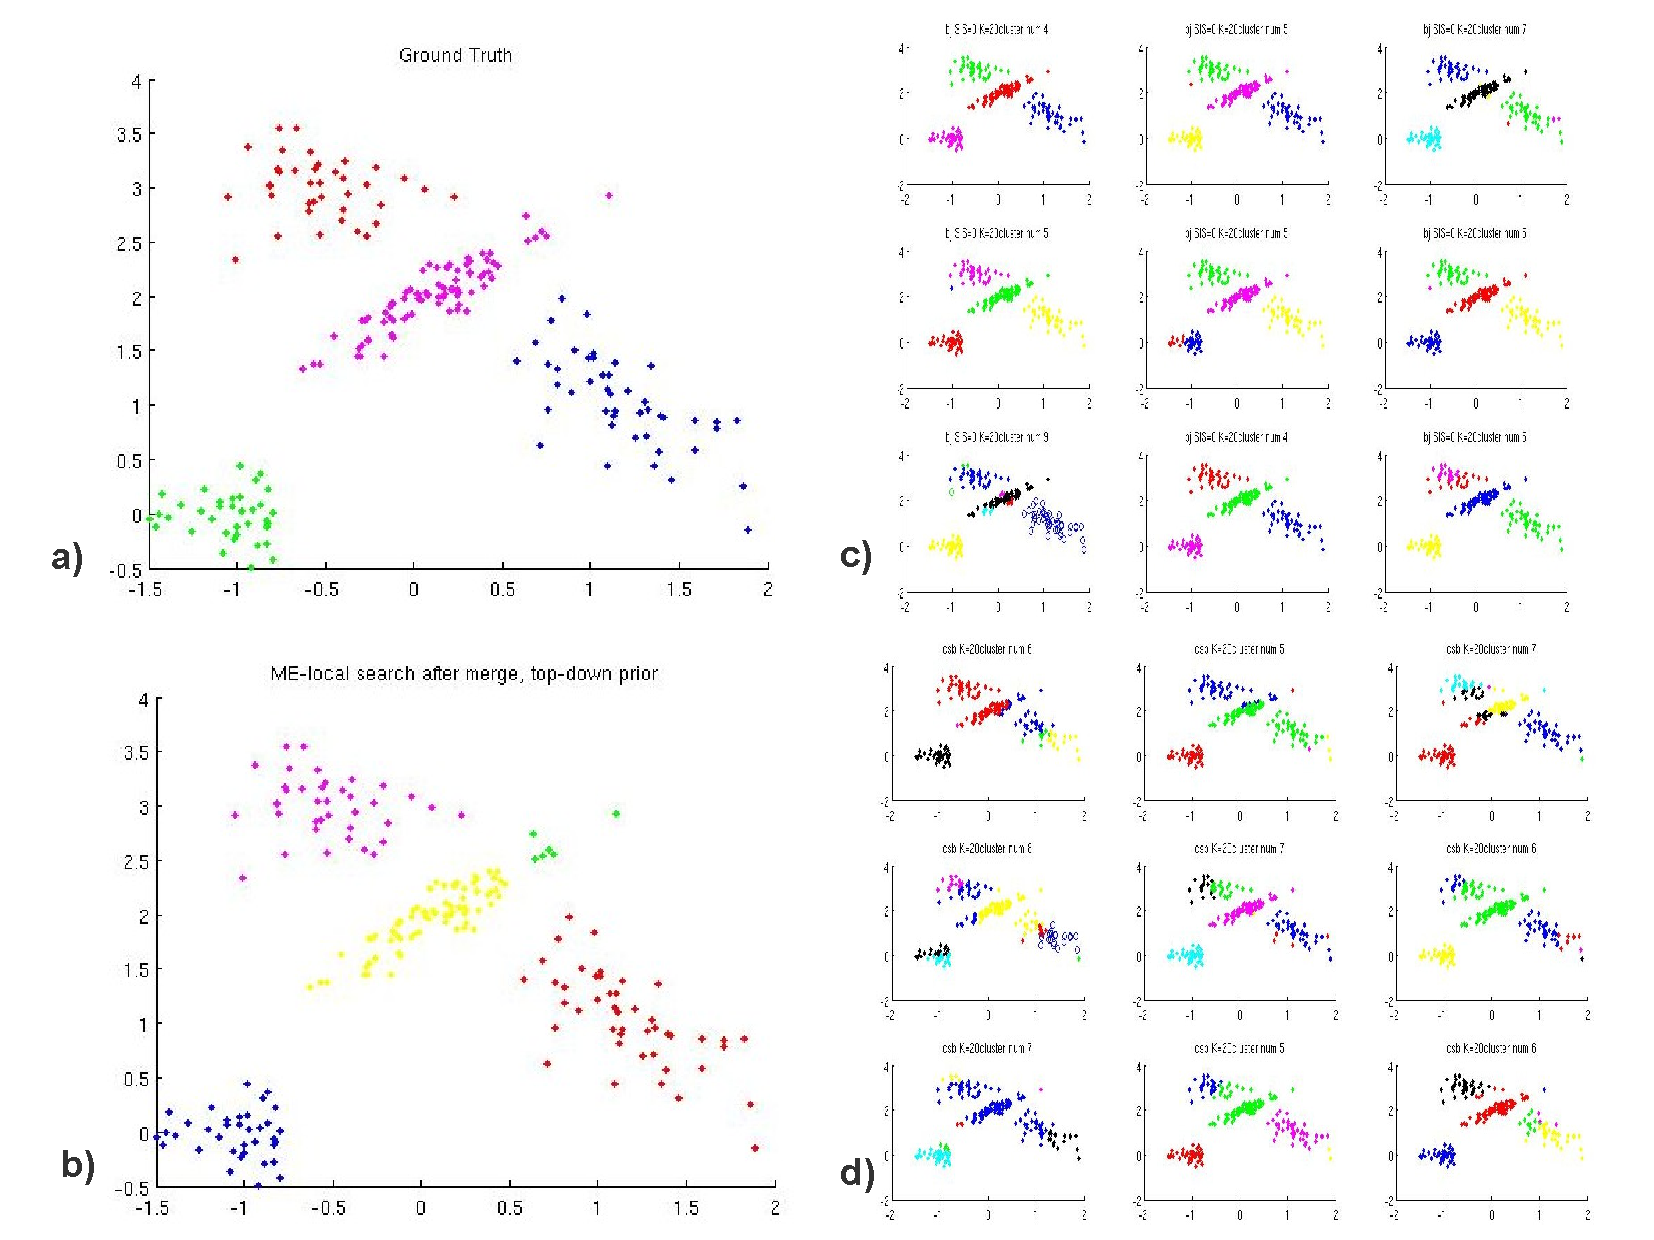
\includegraphics[width=1.0\textwidth]{me_dp.pdf} 
    \caption{a)Ground Truth. b)One run of local search+merge.c)Nine runs for EE.c)Nine runs for Collapsed EE} 
    \label{fig:by:table} 
\end{figure}
\begin{table}[t]
\caption{Comparison of EE, Collapsed-EE and ME algorithms for DP mixture(with mean and std)}
\begin{center}
\begin{tabular}{|l|l|l|l|}
\hline
{\bf Learning Algorithm} &{\bf Initial Cluster Numbers} &{\bf Number of clusters}  &{\bf RandIndex} \\ 
\hline 
\multirow{2}{*}{EE(sampled initialization)} & 10 & 4.1(0.3) & 0.99(0.00) \\
					    & 20 & 4.1(0.3) & 0.99(0.00)\\
\hline
\multirow{2}{*}{EE(random initialization)}  & 10 & 6.9(1.2)&  0.97(0.01) \\
					    & 20 & 7.6(1.7)&  0.93(0.02) \\
\hline
\multirow{2}{*}{Collapsed EE}               & 10 & 5.6(1.6)&  0.90(0.22) \\
					    & 20 & 7.4(0.9)&  0.87(0.09) \\
\hline
\multirow{4}{*}{ME}                         & 1(Top-down) &    4  &  1 \\
					    & 200(Bottom-up) & 4  &  1 \\
					    & 200(Local search) & 15.5(3.9)&  0.83(0.09) \\
					    & 200(Local search+Merge) & 6.5(0.9)&  0.93(0.09) \\
\hline
\end{tabular}
\end{center}
\end{table}
\section{ME algorithm for HDP}
\subsection{Formula}
Here we use the Chinese Restaurant Franchise representation of the HDP. Customer i in restaurant j is associated with an iid draw from $G_j$ and sits at table $t_{ji}$ . 
Table t in restaurant j is associated with an iid draw from $G_0$ and serves a dish $k_{jt}$ from a franchise-wide menu.
Dish k is associated with an iid draw from H. If H is an absolutely continuous measure then each such dish is unique with probability one.
There are $n_{jtk}$ customers in restaurant j sitting at table t and eating dish k, and there are $m_{jk}$ tables in restaurant j serving dish k.\\
Thus the log-likelihood: 
\begin{eqnarray*}
log(p(x,\vec t,\vec k|\lambda))
&=&\underline{\sum_{j=1}^{J} \{log \frac{\Gamma(\alpha)}{\Gamma(n_{j..}+\alpha)}+\sum_{t=1}^{m_{j.}}[log(\Gamma(n_{jt.})+log \alpha
]\}} \\
&+&log \frac{\Gamma(\gamma)}{\Gamma(m_{..}+\gamma)}+\sum_{k=1}^{K} [log(\frac{\Pi_{w=1}^{W}\Gamma(\lambda_{0}+n_{..k}^{w})}{\Gamma(n_{..k}+W\lambda_{0})})+log(\frac{\Gamma(W\lambda_{0})}{\Gamma(\lambda_{0})^{W}})
+log(\Gamma(m_{.k})+log \gamma]\\ 
\end{eqnarray*}
Where $m_{.k}$ is the number of tables in dish k,$m_{j.}$ the number of tables in Restaurant j,
$n_{jt.}$ the number of customers in Restaurant j table t, $n_{j..}$ the number of tables in Restaurant j,
$n_{..k}$ the number of customers in dish k, $n_{..k}^{w}$ the number of tables in dish k with word w.


\subsection{Algorithm}
In general, we make the search algorithm sequential with different levels: customer-level, table-level, restaurant-level and dish-level. Lower level search involves small part of the object function, which is fast in speed while higher level search is the way to get out of local minima in the likelihood space by having a grander view of the landscape.
\\In order to better to explain the advanced randomized search algorithm, we use the bar data test case as an example.
We have 25 different words and each restaurant is represented by a a 5*5 matrix, whose entries are the corresponding counts of the occurence of the word in the restaurant.
The restaurants are generated by 10 dishes corresponding to vertical and horizontal bars and the goal is to find these bars given the restaurants.
\begin{enumerate}[(a)]
\item {\bf Local-Customer,Local-Table}\\
\emph{Description}:\\
Local-Customer: fixing others, find the best table assignment for a customer\\
Local-Table: fixing others, find the best dish assignment for a table\\\\
\emph{Reasoning:}\\ In the literature on the inference of HDP model, Gibbs Sampler(Teh et.al.2006) is the most popular one.
Start from the Gibbs Sampler with Chinese Restaurant Franchise Representation, we propose the corresponding deterministic search methods.\\
\item{\bf Merge-Table}\\
\emph{Description}:\\
Merge-Table:fixing others, find the best table for a certain table to merge\\ \\
\emph{Reasoning:}\\
Shown in figure 2.b), sometimes change one customer at a time may be worse-off but merge them will improve the log probability.
\item {\bf Decompose-Restaurant}\\
\emph{Motivation}:\\
Inherited from the algorithm for DPM model, we need a move to split a certain table into two by k-means++\\ 
Shown in figure 2.a), if we start with only one table, local/merge moves won't divide it into two tables.\\
But it's usually hard to determine k for k-means++ which is also costly.\\\\
\emph{Description}:\\
Decompose Restaurant:fixing others, approximate the best configuration for a restaurant by: Initialization+Merge-Table+Local-Customer+Local-Table.\\ 
Initialization: Remove previous configuration related to the restaurant and heuristically sample to form tables according to the dishes.\\\\
\emph{Reasoning:}\\
Shown in figure 2.c), if start from a bad configuration, even split or move will get stuck.
We'd better reconfigure it over instead of making fancier moves by combining different moves together.
\item {\bf Local-Dish}\\
\emph{Description}:\\
Local-Dish: fixing others, find the best dish assignment for a word\\\\
\emph{Reasoning:}\\Previously, we are working on the restaurant-level without direct concern of the dish configuration which is really the answer we want.
Shown in figure 2.d), sometimes the overlapped part of two dishes is only assigned to one of the bars. Thus we need a move to configure a single word across restaurants.
\item {\bf Merge-Dish}\\
\emph{Description}:\\
Merge-Dish:fixing others, find the best dish for a certain dish to merge\\ \\
\emph{Reasoning:}\\Similar to Merge-Table.
\item {\bf Decompose-Dish}\\
\emph{Description}:\\
Decompose Dish:fixing others, approximate the best configuration for a dish by: Initialization+Merge-Dish+Local-Dish.\\ 
Initialization: Remove previous configuration related to the dish and decompose the restaurants that previously have tables in the dish.\\\\
\emph{Reasoning:}\\Similar to Decompose Restaurant.
\end{enumerate}
\begin{figure}[h] 
  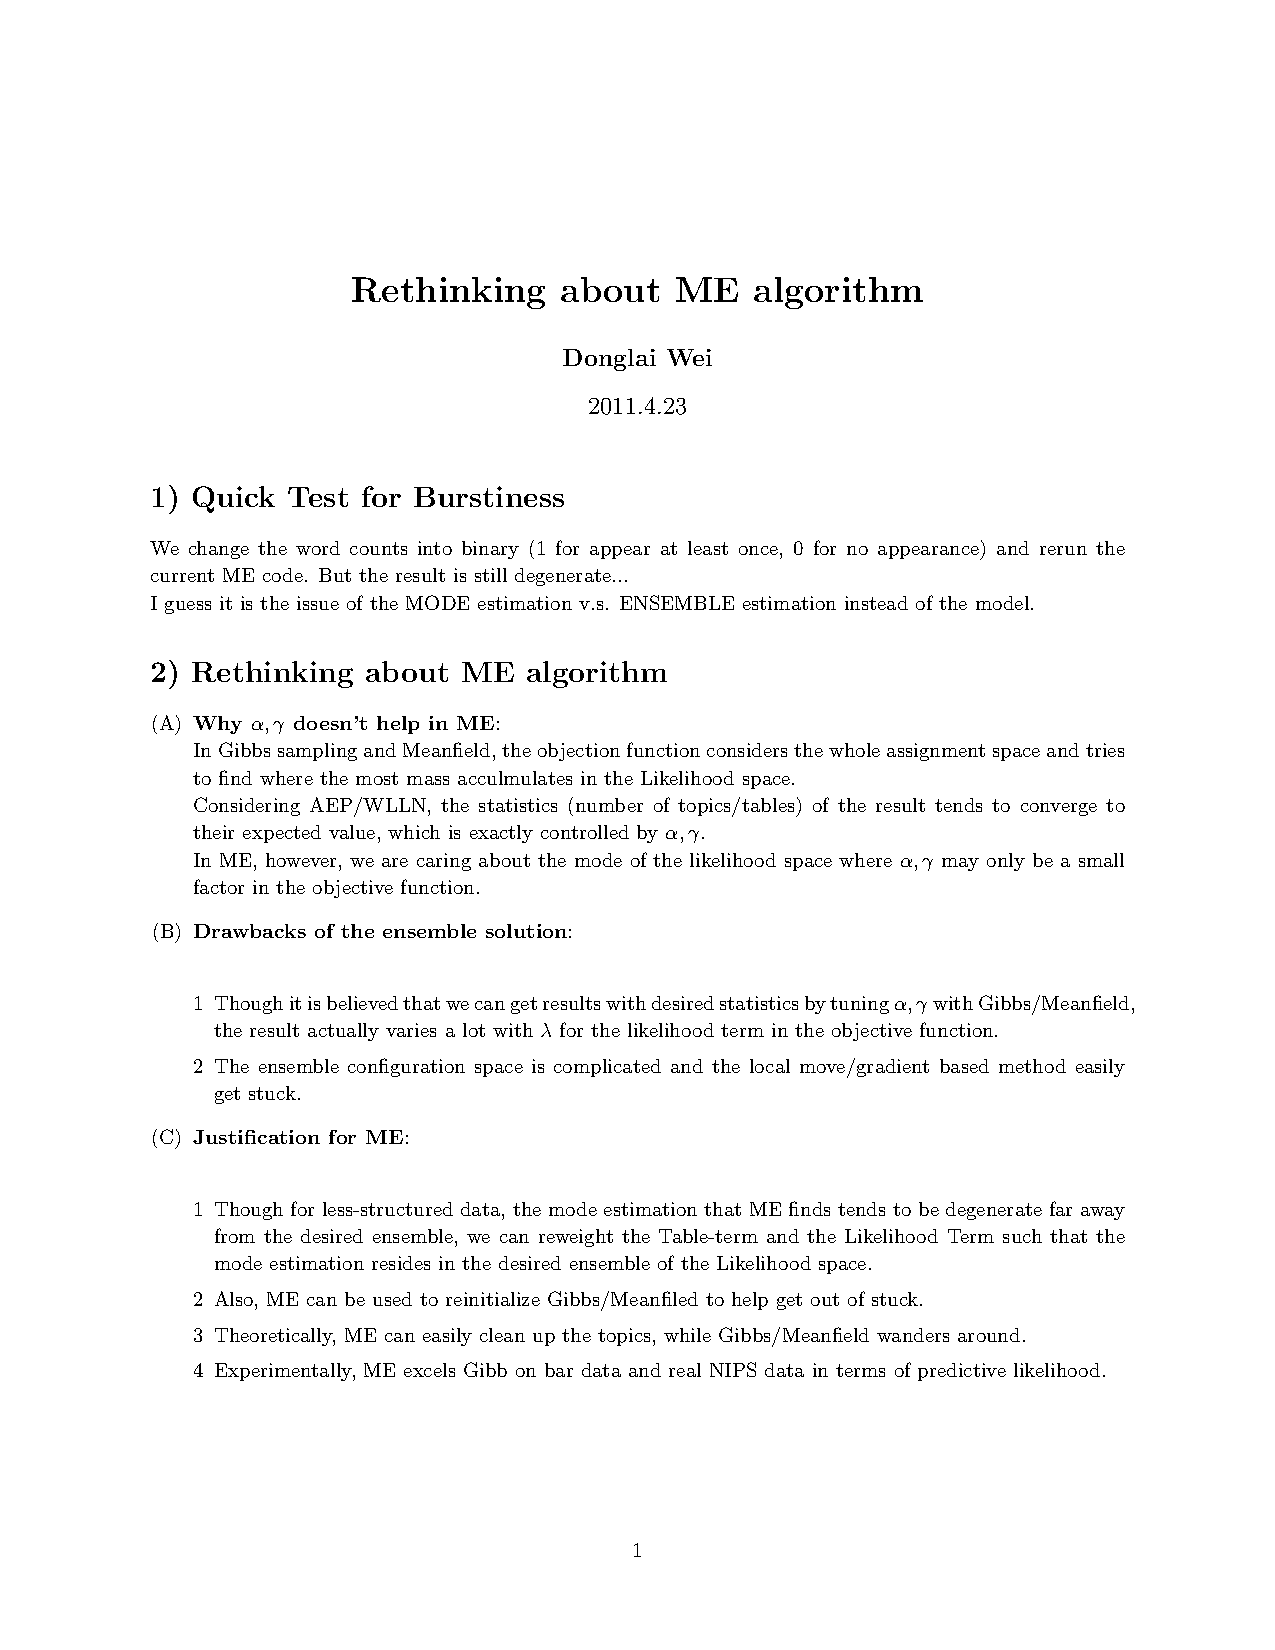
\includegraphics[width=2in,height=2in]{me.jpg} 
  \caption{a)configuration of a restaurant in the Bar test b)Reason for Merge move c)Reason for Decompose move.d)Reason for Local-Dish move} 
  \label{fig:by:table} 
\end{figure}


\subsection{Results}
\subsubsection{Test on Bar data}
Here, we do the Bar data test described above to compare our ME algorithm with the crf and block Gibbs Sampler in [7].
There are 200 restaurants (5$\times$5 matrix), each of which has 50 customers.
We set the same hyperparameters for these three algorithms and run 1000 iterations for each Gibbs Sampler while running ME to convergence.
Figure 3a) shows the comparison of the final configuration of the dish detected. 
Clearly, ME algorithm is more efficient to improve noisy dish by deterministic searches while samplers may take long to figure it out.
Figure 3b) shows the comparison of the log-likelihood for one run of ME algorithm and 10 runs for each Samplerm where ME algorithm finds the higher log-likelihood.
\begin{figure}
 \centering
   \begin{tabular}{cc}    
     \resizebox{50mm}{!}{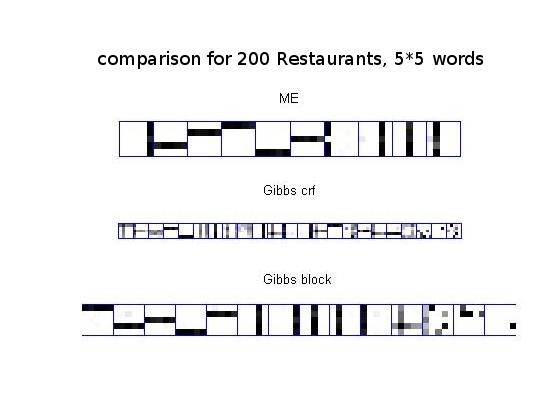
\includegraphics{200_con.jpg}} &
     \resizebox{50mm}{!}{\includegraphics{200_con_l.jpg}} \\
   \end{tabular}
    \caption{a)Configuration Comparison ;b)Likelihood Comparison}
    \label{fig:by:table} 
\end{figure}

\subsubsection{Test on NIPS abstract Data}
Here, we take a subset of the NIPS abstract Data set from the topic model toolbox in Matlab.
This subset contains 100 different words and 200 documents, each of which has around 200 data points.
We compare the performance of LDA,LDA-HMM from the toolbox, crf and block Gibbs Sampler in [7] and our ME algorithm.
So far, I don't know how to evaluate the performance.

\section{Extensions for HPY}
The modification of the formula from HDP to HPY is trivial, where only four terms in the log-likelihood formula need to be changed.\\
$log(p(x,\vec t,\vec k|\lambda))$
\begin{eqnarray*}
&=&\sum_{j=1}^{J} \{log \frac{\Gamma(\alpha+dm_{j.})}{\Gamma(n_{j..}+\alpha)}+\sum_{t=1}^{m_{j.}}[log(\frac{\Gamma(n_{jt.}-d)}{\Gamma(1-d)})]\} \\
&+&log \frac{\Gamma(\gamma)}{\Gamma(m_{..}+\gamma)}+\sum_{k=1}^{K} [log(\frac{\Pi_{w=1}^{W}\Gamma(\lambda_{0}+n_{..k}^{w})}{\Gamma(n_{..k}+W\lambda_{0})})+log(\frac{\Gamma(W\lambda_{0})}{\Gamma(\lambda_{0})^{W}})
+log(\frac{\Gamma(m_{.k}-\eta)}{\Gamma(1-\eta)})+log\frac{\Gamma(\gamma+K\eta))}{\Gamma(\gamma)}]\\ 
\end{eqnarray*}
\section{Discussion}
In Chinese Restaurant Franchise Representation, there are only t-term and k-term in the object function.
If start from a decent initialization(say, from Gibbs sampler) where t-term and k-term are equally ok, then the ME algorithm we proposed can find the solution efficiently.
But if the initialization strongly favors one term over another, we will need annealing schedule to weight two terms in the object function gradually to get out of the local minima.  
\section{Conclusion}
In this report, we first show the advantage of ME alogorithm over other variational methods to learn Dirichlet Process Mixture Model. Later we 
develop the randomized ME algorithm for Hierarchical Dirichlet Process Model, which works reasonably well on the toy data. Our future 
direction is to improve and test the algorithm on real data sets for document classification and natural image segmentation.c


\section{References}
\small{
[1]  Blei,D,M, Jordan,M.I, and Ng, A. Y. (2003), “Hierarchical Bayesian Models for Applications 
  in Information Retrieval,” in Bayesian Statistics, vol. 7, pp. 25–44 

[2] E.B.Sudderth and M.I.Jordan(2008)Shared Segmentation of Natural Scenes Using Dependent Pitman-Yor Processes NIPS 2008


[3] Ghahramani, Z. and Beal, M. J. (2000). Variational inference for Bayesian mixtures of                                                          ̈
  factor analysers. In S. A. Solla, T. K. Leen, \& K.-R. Muller (Eds.), Advances in neural
  information processing systems, 12. Cambridge, MA: MIT Press.

[4] K. Kurihara and M. Welling. Bayesian K-means as a
 ”maximization-expectation” algorithm. Neural Computation, 2008

[5] Y. W. Teh, K. Kurihara and M. Welling. Collapsed Variational Inference for HDP
NIPS 2007

[6] Y. W. Teh and M.I.Jordan.Hierarchical Bayesian Nonparametric Models with Applications.(2010) Bayesian 
Nonparametrics in Practice, Cambridge, UK: Cambridge University Press.

[7] Y. W. Teh, M. I. Jordan, M. J. Beal, and D. M. Blei. Hierarchical Dirichlet processes. Journal of the 
American Statistical Association, 101(476):1566–1581, 2006.

}
\section{Appendix: Pseudocode of ME algorithm for HDP}
J restaurants,K dishes
\subsection{Backbone}
\begin{alltt}
  \(\%a)Initialization:\)
      Every restaurant has only one table and its own dish
  \(\%b)Annealing:(n:number of iterations; p:annealing power)\)
      For iter=1:n
          Temperature=\((\frac{iter}{n})^p\)
          Decompose Dish(Temperature)
      End
  \(\%c)Run for Convergence:\)
      While L doesn't increase any more:          
          For j=randperm(J):
              Decompose restaurants(j,1,0)
          End
          Decompose Dish(1)
      End
\end{alltt}
\subsection{Decompose Dish(Negative Temperature:Temperature)}
\begin{alltt}
For k=Randperm(K)

   \(\%a)Initialization: Reconfig without Dish k\)
      For j=restaurants which have tables serving dish k
          Decompose Restaurant(j,Temperature,k);
      End

   \(\%b)Merge new proposed dishes+Local-Dish\)
      For k=new proposed dishes
          Merge Dish(Temperature,k);
      End     
      For w=words which appear in dish k
          Local-Dish(w,Temperature,k);
      End 

   \(\%d)Decision\)
      If(\(\Delta k-term+\Delta w-term+{\bf Temperature}*\Delta t-term<\)0):
          Accept new config
      End
End
\end{alltt}
\subsection{Decompose restaurants(Restaurant index:$j$,Negative Temperature:$T$,The Decomposed Dish: $k_{0}$)}
\begin{alltt}
\(\%a) Initialization\)
Make Restaurant j into one table \(t\textsubscript{0}\) where customers following uniform distribution
\(\%(P(t\textsubscript{ji}=t\textsubscript{0})=\frac{1}{W})\)      
Possible Dish=\(\{Nonempty \ dishes\}\setminus k\textsubscript{0}\)      
While Possible Dish is not empty:      
      For each dish \(k\in\)Possible Dish:          
          For each customer i in \(t\textsubscript{0}\):
              sample \(t\textsubscript{ji}\in\{t\textsubscript{0},t\textsubscript{k}\}\sim\{\frac{1}{W},\frac{n\textsubscript{..k}\textsuperscript{w}+\phi}{n\textsubscript{..k}+W\phi}\}\)                
          End
      Propose to form table \(t\textsubscript{k}\) with customers whose \(t\textsubscript{ji}=t\textsubscript{k}\)
      Calculate the change \(d\textsubscript{k}\) for k-term and w-term:
      End
      \(\%\)Sample a proposal \(t\textsubscript{k*}\) according to the weight and make the new table:
      Sample a proposal \(\{t\textsubscript{k\textsubscript{1}},...,t\textsubscript{k\textsubscript{K}}\}\sim e\textsuperscript{r\textsubscript{proposal}\{d\textsubscript{k\textsubscript{1}},...,d\textsubscript{k\textsubscript{K}}\}}\)
      \(\%r\textsubscript{proposal}>0\), the more decrease of \(d\textsubscript{k}\), the less propable to form table \(t\textsubscript{k}\)
      Possible Dish=Possible Dish\(\setminus k\textsubscript{*}\)
      \(t\textsubscript{0}=t\textsubscript{0} \setminus t\textsubscript{k\textsubscript{*}}\)
End
If there are still customers left in \(t\textsubscript{0}\):
   make it a new table with a new dish K+1
End

\(\%\)b)Refinement for Restaurant j(Local-Search and Merge Move for tables in Restaurant j)
LM-Restaurant(j,T)

\(\%\)c)Decision
Calculate the change of L between present Restaurant j config and its previous config: 
\(\Delta L'=\Delta k-term+{\bf T}\Delta t-term+\Delta w-term\)
If(\(\Delta L'<\)0):
    Accept the new configuration
Else:
    Restore Previous Config
End    
\end{alltt}
\subsection{LM-Restaurant(Restaurant index:$j$,Negative Temperature:$T$)}
\begin{alltt}
While L doesn't increase any more:
     
     \(\%\)a)Local-Customer:
        For t\textsubscript{1}=Randperm(m\textsubscript{j.}):
             For t\textsubscript{2}=Randperm(m\textsubscript{j.}\(\setminus\) t\textsubscript{1}):
                While local move can be made:
                      Greedily move one customer at a time from \(t\textsubscript{1}\) to \(t\textsubscript{2}\) if the move increases {\bf L'(T)} 
                End
             End
        End
     
      \(\%\)b)Local-Table:
        For \(t\textsubscript{1}\)=Randperm(\(m\textsubscript{j.}\)):
            Assign \(t\textsubscript{1}\) to the dish which increase L most(allow it to have new dish)
        End
              
      \(\%\)c)Merge Table:
        For \(t\textsubscript{1}\)=Randperm(\(m\textsubscript{j.}\)):
            Merge table \(t\textsubscript{1}\) to the table in j with the best dish k, which increase \({\bf L'(T)}\) most
            \(\%\)if cannot increase L'(T),then leave it alone
        End

End
\end{alltt}
\subsection{v) Merge-Dish(Dish index:$k$,Negative Temperature:$T$)}
\begin{alltt}
Dish List=\(\{Nonempty \ dishes\}\setminus k\)
 
While Dish List is not empty:
    Randomly pick a dish k\(\in\) Dish List
    Dish List=Dish List\(\setminus\)k
    Merge dish k to the dish\(\in\) Dish List which increase \({\bf L'(T)}\) mostly
    \(\%\)if cannot increase L'(T), then leave it alone
End
 
\end{alltt}
\subsection{Local-Dish(Dish index:$k$,Negative Temperature:$T$)}
\begin{alltt}
Dish List=\(\{Nonempty \ dishes\}\setminus k\)

For w=Randperm(Words Occur in Dish k):
    
    \(\%\)i) Find promising dishes(appear most often with the tables having word w in dish k)
    For kk=Dish List
        Restaurant_index(kk)=index of restaurants in dish kk, that have tables serving dish k       
        Restaurant_count(kk)=length(Restaurant_index(kk))
    End 
    Promising_Dishes=find(Restaurant_count==max(Restaurant_count))

    \(\%\)ii) Find the best approximated Reallocation of word w:
    \(\Delta L\)=0; 
    For kkk=Promising_Dishes: 
	
         \(\%\)a)Naive Reallocation:	
        For j=Restaurant_index(kkk)
            Assign all of words w from the table serving dish k to the table serving dish kkk
        End
        Calculate the change of L between present config and previous config:\(l\textsubscript{0}\)
	
        \(\%\)b)Gready Search:
        \(\Delta l\)=1
        While \(\Delta l>\)0
              \(\Delta l\textsubscript{k}\)=\(\Delta K\)(assign one word w from dish kkk back to dish k)
              \(\Delta l\textsubscript{t}\)=max(\(\Delta T\)(assign one word w from dish kkk back to dish k in Restaurant j\(\in\)Same Restaurant(kkk)))
              \(\Delta l=\Delta l\textsubscript{k}+\Delta l\textsubscript{t}\)
        End
        \(\Delta L=max(\Delta L,l\textsubscript{0}+\Delta l)\)
    End 

    \(\%\)iii)Decision:
    If \(\Delta L>\)0
        Accept new config
    Else
        Restore previous config
    End 
End 
\end{alltt}

\end{document}
